\documentclass[12pt, notitlepage]{article}
\usepackage{amsmath}
\usepackage{amssymb}
\usepackage{graphicx}
\usepackage{amsthm}
\usepackage{listings}
\usepackage{color}
\usepackage{epstopdf}
\usepackage{float}

\definecolor{dkgreen}{rgb}{0,0.6,0}
\definecolor{gray}{rgb}{0.5,0.5,0.5}
\definecolor{mauve}{rgb}{0.58,0,0.82}

\lstset{
	frame=single,
	language=Java,
	belowskip=3mm,
	showstringspaces=false,
	columns=flexible,
	captionpos=b,
	basicstyle={\small\ttfamily},
	numbers=left,
	numbersep=5pt,
	%numbers=none,
	numberstyle=\tiny\color{gray},
	keywordstyle=\color{blue},
	commentstyle=\color{dkgreen},
	stringstyle=\color{mauve},
	breaklines=true,
	breakatwhitespace=true,
	tabsize=3
}


\providecommand{\abs}[1]{\lvert#1\rvert}
\providecommand{\norm}[1]{\lVert#1\rVert}

\newtheorem{thm}{Theorem}
\newtheorem{lemma}[thm]{Lemma}
\newtheorem{fact}[thm]{Fact}
\newtheorem{cor}[thm]{Corollary}
\newtheorem{eg}{Example}
\newtheorem{ex}{Exercise}
\newtheorem{defi}{Definition}
\newtheorem{hw}{Homework}
\newenvironment{sol}
  {\par\vspace{3mm}\noindent{\it Solution}.}{\qed}

\newcommand{\fib}{\mbox{fib}}
\newcommand{\ov}{\overline}
\newcommand{\cb}{{\cal B}}
\newcommand{\cc}{{\cal C}}
\newcommand{\cd}{{\cal D}}
\newcommand{\ce}{{\cal E}}
\newcommand{\cf}{{\cal F}}
\newcommand{\ch}{{\cal H}}
\newcommand{\cl}{{\cal L}}
\newcommand{\cm}{{\cal M}}
\newcommand{\cp}{{\cal P}}
\newcommand{\cz}{{\cal Z}}
\newcommand{\eps}{\varepsilon}
\newcommand{\ra}{\rightarrow}
\newcommand{\la}{\leftarrow}
\newcommand{\Ra}{\Rightarrow}
\newcommand{\dist}{\mbox{\rm dist}}
\newcommand{\bn}{{\mathbf N}}
\newcommand{\bz}{{\mathbf Z}}

\setlength{\parindent}{0pt}
%\setlength{\parskip}{2ex}
\newenvironment{proofof}[1]{\bigskip\noindent{\itshape #1. }}{\hfill$\Box$\medskip}

\usepackage{enumerate,fullpage, proof}
\newcommand{\Infer}[2]{\infer{#2}{#1}}

\title{Homework 5}
\author{Team: nogg\footnote{E-mail: \texttt{kimi.ysma@gmail.com}}\footnote{Team member: Ma Yesheng, Zhao Ming, Hu Hu, Zou Yikai, Fan Minghua}}

\begin{document}

{\bf\small CS214: Algorithms and Complexity}\hfill{\bf\small 2016 Fall}
{\let\newpage\relax\maketitle}

\textbf{Solution 1:}\\

\textbf{Solution 2:}\\
\begin{enumerate}[1.]
\item Since in a cycle of $n$ edges, a mincut can only contain $2$ edges
    and we can choose the $2$ edges from $n$ edges. Thus the number of
        mincuts in a $C_n$ should be $\binom{n}{2}$
\item Suppose we there are $m$ different global mincuts. For the Karger's algorithm, the probability of each global mincut
    should be $\frac{1}{\binom{n}{2}}$ and since these are all disjoint events we get:
        \[
            \sum_{1}^{m} \frac{1}{\binom{n}{2}} \leq 1
            \]
        Thus we get that the max kinds of mincut should be $\binom{n}{2}$.

\item Simply consider that for $s$, we have $v_1, v_2 \ldots v_n$ connected to $s$ and we also have these
    $v_1, v_2 \ldots v_n$ connected to $t$. Since $s$ and $t$ has to be in different $S$ and $\overline{S}$,
    we can arbitrarily take $v_i$ to $S$ or $\overline{S}$ without changing the value of mincut, which should be $n$.
    In this we, we the total number of mincuts should be $2^n$, which is a exponential number.
\end{enumerate}


\textbf{Exercise 3.}
\begin{sol}

Here is the example based on which we cannot find a maximum cut from the modified Stoer-Wagner algorithm. This is the initial undirected-weighted graph.\\
\begin{figure}[H]
	\centering
	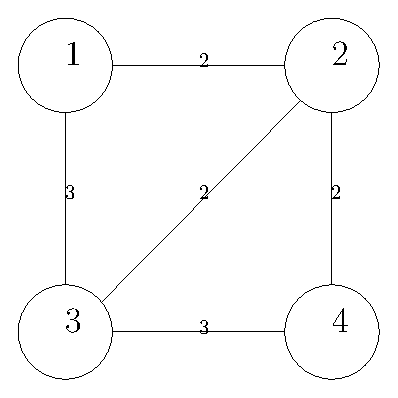
\includegraphics[width=0.4\linewidth]{1.eps}
\end{figure}

Based on the modified algorithm, we will choose the least tightly connected vertex.\\
So we choose vertex from 1 vertex.\\
And the cut phase will be {1, 2, 4} {3}. In the meantime, the weight is 2 + 3 + 3 = 8. And we merge the vertex 4 and 3. The remaining graph is as followed.\\

\begin{figure}[H]
	\centering
	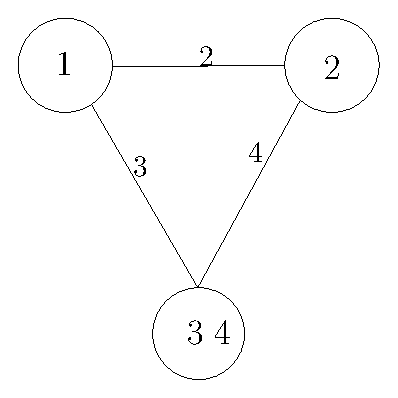
\includegraphics[width=0.4\linewidth]{2.eps}
\end{figure}

And continuing, the cut phase will be {1, 2} {3 4}. The weight is 3 + 4 = 7. And merge 2 and 3 4. The remaining graph is as followed.\\

\begin{figure}[H]
	\centering
	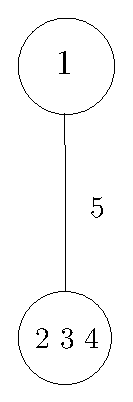
\includegraphics[width=0.1\linewidth]{3.eps}
\end{figure}

The weight is 5.\\
As a result, the max weight we get from the modified algorithm is 8. However, if we consider the cut {1, 4} and {2, 3}, the weight is 3 + 3 + 2 + 2 = 10. So the result is wrong. So the modified Stoer-Wagner Algorithm fails to find the maximum cut.\\
\end{sol}

\end{document}
